% !TEX encoding = UTF-8
% !TEX TS-program = pdflatex
% !TEX root = ../tesi.tex

%**************************************************************
\chapter{Svolgimento del progetto}
\label{cap:ilprogetto}
%**************************************************************

% \intro{Breve introduzione al capitolo}

%**************************************************************
\section{Analisi e pianificazione}

\subsection{Analisi}
Il mio stage è iniziato quando ormai l'analisi era finita, quindi non ho avuto nessun contatto con il proponente. Tuttavia sono stato messo subito al corrente dei
requisiti individuati e sono stati inseriti negli obiettivi del progetto di stage, quindi già esplicati nel capitolo precedente. Essendo un refactoring di un applicazione
già esistente parte dei requisiti erano già stati stabiliti, quindi elencherò i principali cambiamenti richiesti. Utilizzerò come notazione R+(F|Q|V)+X+(D|O), dove:

\begin{itemize}
  \item R: requisito;
  \item F: funzionale;
  \item Q: qualitativo;
  \item V: di vincolo;
  \item X: numero progressivo;
  \item D: desiderabile;
  \item O: obbligatorio;
  \item Z: opzionale.
\end{itemize}

Alcuni dei requisiti più importanti individuati sono riportati nella tabella \autoref{tab:requisiti}, con codice e relativa descrizione:

\renewcommand{\arraystretch}{2}
\begin{longtable}{|p{4cm}|p{10cm}|}%
  \caption{Tabella del tracciamento dei requisti funzionali} 
  \label{tab:requisiti} \\
  
    \hline
    \textbf{Requisito} & \textbf{Descrizione} \\
    \hline
    \endhead
    RF1O     & L'interfaccia permette di fare il login nel sistema gestionale di UCIS \\ \hline
    RQ2O     & L'applicazione riconosce se è già stato effettuato un login e utilizza i dati salvati per effettuarlo \\ \hline
    RQ3O     & L'applicazione deve funzionare offline se la persona è già autenticata \\ \hline
    RV5O     & I dati dell'account non vanno salvati nella memoria, ma nel sistema Android \\ \hline
    RF8O     & L'interfaccia permette di creare attività \\ \hline
    RF9O     & L'interfaccia permette di visualizzare un'attività \\ \hline
    RF10O     & L'interfaccia permette di avviare la registrazione di un'attività \\ \hline
    RF11O     & L'avvio di un attività provoca l'invio di log che registrano la posizione dello smartphone \\ \hline
    RF12O     & L'applicazione invia i log registrati al sistema gestionale UCIS \\ \hline
    RV18O     & L'applicazione deve essere scritta con uno strumento che permetta lo stesso codice per tutte le piattaforme \\ \hline
\end{longtable}%

%**************************************************************

\subsection{Studio di Fattibilità}

\subsubsection{Framework per lo sviluppo mobile}
Come specificato dal requisito RV18O si era alla ricerca di un framework crossplatform. Di seguito alcune delle tecnologie che abbiamo analizzato e alcuni dei motivi per
cui non sono stati scelti.

\paragraph{Cordova e PhoneGap}

\begin{figure}[h]
	\begin{center}
		
\includegraphics[height=2.5cm]{cordova}
		\caption{Logo di Cordova}
	\end{center}
\end{figure}

La prima tecnologia con cui sono stato a contatto è stato il framework Cordova. Il software è stato acquisito da Adobe nel 2011 mantenendolo \gls{open source} e
rilasciandolo nel 2013 con il nome di Apache Cordova. Stiamo parlando di un framework che permette attraverso alcuni tools di creare applicazioni utilizzando CSS3, HTML5 e
Javascript, evitando allo sviluppatore di affidarsi alle API specifiche del sistema operativo. Il pregio di questa tecnologia è il fatto che la stessa
applicazione non dovrà essere scritta in Java per Android, in XCode o Swift per iOS, ma avrà un codice unico che sarà adattato per i singoli sistemi operativi. \\
Tutto ciò funziona tramite le WebView native. Le WebView sono delle componenti delle applicazioni utilizzate per visualizzare contenuti web. Queste sono
sviluppate dai sistemi operativi e non fanno altro che renderizzare ciò che è stato scritto con linguaggio HTML5, CSS3, Javascript. Per facilitarne la
comprensione si possono immaginare come delle pagine web visualizzate all'interno di un browser, senza gli elementi tipici di esso (come la barra dell'URL,
delle tab o le opzioni). \\
Le applicazioni sviluppate in questo modo si possono considerare sia in parte \gls{web-based}, sia in parte native perché utilizzano e hanno accesso a tutti i componenti
hardware della piattaforma sulla quale vengono eseguite. Ciò avviene tramite i plugin, che possono essere parte del framework, oppure, tramite API apposite,
scritti dallo sviluppatore stesso. Inoltre l'applicazione può essere impacchettata, installata o caricata negli store ufficiali come una qualunque altra nativa.
\\
La forza di Cordova e del fatto che sia open source, sta nel fatto che possiede una libreria vastissima di plugin utilizzabili che forniscono un controllo
totale sul dispositivo, come se si sviluppasse dal linguaggio nativo. Uno dei plugin che abbiamo immediatamente ricercato, è quello che si occupa del
tracciamento GPS continuo in \gls{background}. Siamo andati quindi a creare un primo prototipo di applicazione installando solamente quel plugin per semplice
test. Durante questo veloce procedimento abbiamo però riscontrato diversi problemi nell'installazione delle varie componenti o nella compatibilità con altre
librerie (come nel nostro caso con le \gls{SDK} di Android). L'impressione di questo software non è stata positiva, perché mi è sembrato vecchio
e poco mantenuto. Informandomi poi ho notato che le varie aziende, che lo utilizzavano come framework di sviluppo si stavano muovendo su altri software nuovi e
più aggiornati.\\
Menzione d'obbligo è da fare ad Adobe PhoneGap, nato come versione non \gls{open source} di Cordova, che fornisce a pagamento servizi molto interessanti, come ad
esempio la build in cloud dell'applicazione, eliminando i problemi derivati dall'ambiente di sviluppo sul quale si sta lavorando.

\paragraph{Ionic e Capacitor}

\begin{figure}[h]
	\begin{center}
		
\includegraphics[height=2.5cm]{ionic}
		\caption{Logo di Ionic}
	\end{center}
\end{figure}

Ionic è un framework open-source rilasciato da Drifty Co. nel 2013. La prima versione di Ionic non era altro che un SDK che metteva a disposizione una
piattaforma AngularJS per lo sviluppo di applicazioni con Cordova. Le ultime versioni di Ionic hanno aggiunto nuove funzionalità, tra le
quali la possibilità di scegliere di sviluppare in Angular, React o Vue. Inoltre è stato rilasciato un software per la build e le API proprietario,
chiamato Capacitor, che racchiude al suo interno Cordova, aggiornandolo e adeguandolo alle nuove SDK dei vari Sistemi Operativi. Perciò derivando
da Apache Cordova, contiene tutte le sue funzionalità, e di conseguenza tutti i suoi pregi, ma anche alcuni dei suoi difetti. \\
Testando Ionic mi sono accorto di alcuni punti deboli delle applicazioni ibride. \\
In primo luogo le performance. Le applicazioni ibride hanno bisogno della WebView che non è altro che un altro processo di supporto per
renderizzare pagine web. Inoltre è un dato di fatto che le applicazioni web sono molto esose dal punto di vista delle risorse rispetto a un
applicazione scritta in linugaggio nativo per quel dato sistema operativo. In secondo luogo non si ha controllo totale sui plugin che
servono a interfacciarsi con il dispositivo. Le librerie native sono molto più ricche e specifiche, ma soprattutto non richiedono
l'intervento di software di terze parti, come Ionic e Capacitor, per funzionare. Questi problemi sono emersi subito, una volta installato
ionic e fatto una veloce build dell'applicazione ci siamo accorti della poca reattività su dispositivi datati e della difficoltà nel
personalizzare i plugin messi a disposizione. \\

\begin{wrapfigure}{l}{0.45\textwidth}
  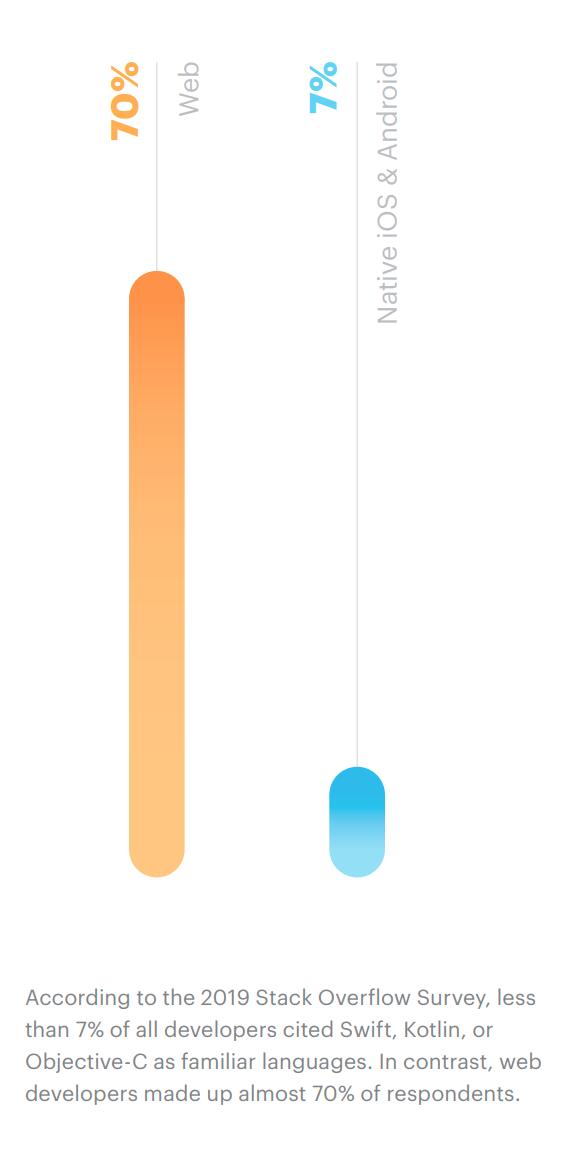
\includegraphics[width=0.9\linewidth]{sviluppatori} 
  \caption{Caption1}
  \label{fig:sviluppatori}
\end{wrapfigure}

Da alcune ricerche da noi effettuate è emerso che la maggior parte delle aziende che sviluppano per mobile si stanno muovendo verso le
applicazioni ibride. I motivi non sono difficili da comprendere. Il fatto che un unico codice può essere eseguito su diversi dispositivi è
sicuramente un fattore molto importante. Finora le aziende dovevano sviluppare applicazioni diverse quindi moltiplicando il costo e le
risorse. Supponendo di utilizzare solo linguaggi nativi, \acrlong{asd} avrebbe dovuto sviluppare almeno due appplicazioni differenti, una
per Android e una per iOS, riutilizzando pochissimo codice e impiegando almeno il doppio di risorse. Sarebbero stati necessari almeno altri
due sviluppatori e i tempi di fornitura sarebbero stati decisamente più lunghi. \\
Inoltre gli sviluppatori con esperienza in API native non sono molto comuni. Non sono rari invece sviluppatori web, dei quali fa parte anche il mio
tutor, come dimostra la figura \autoref{fig:sviluppatori}. \\
Da notare anche come il mondo si stia muovendo molto velocemente verso il web. Moltissime delle applicazioni tuttora si basano su tecnologie
che sono sviluppate per esso, come AWS di Amazon, Azure di Microsoft, Google Cloud e molti altri. Sviluppare in questo senso è
anche un investimento su un mondo che è aperto a opportunità continue e di conseguenza al futuro.

\paragraph{Flutter e Xamarin}
Nonostante mi ritenessi soddisfatto dell'impressione di Ionic, ho preso in cosiderazione un'ultima alternativa, Flutter. \\
Flutter è un framework che si occupa della creazione di interfacce grafiche native per iOS, Android e desktop. Sviluppato da Google e
rilasciato nel 2018, utilizza un linguaggio proprietario Dart, presentato come alternativa a Javascript. L'engine, sviluppata in
\gls{C++}, si occupa di renderizzare i widget, oggetti grafici scritti dallo sviluppatore. Le applicazioni in Flutter quindi possono essere
eseguite su tutti i dispositivi nei quali è presente la VM di Dart e il suo motore grafico. Attualmente questi sono implementati in iOS e
Android e su alcuni browser. \\

\begin{figure}[h]
  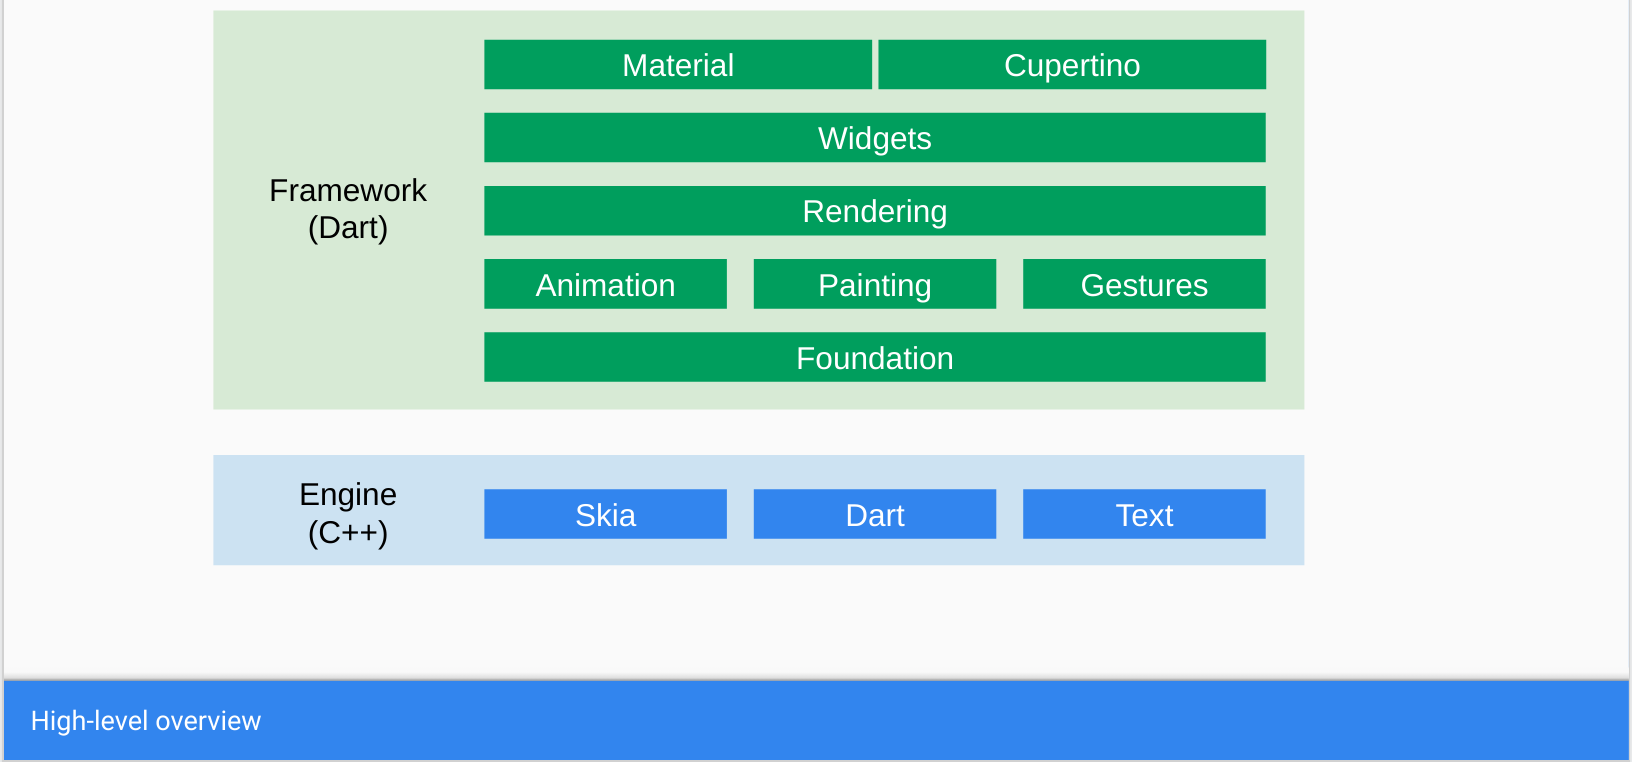
\includegraphics[width=0.9\linewidth]{flutterframe} 
  \caption{Architettura di Flutter}
  \label{fig:flutter}
\end{figure}

L'ovvia conseguenza di questo approccio sono le migliori prestazioni rispetto alle applicazioni web-based, eseguite su una WebView.
Tuttavia il problema riscontrato in questo tipo di tecnologia è il fatto che si dovesse utlizzare un linguaggio proprietario, Dart, che
fosse utile solo al campo dello sviluppo mobile. Inoltre tutti i lati positivi di un framework web non valgono anche in questo caso. Di
fatto l'unica cosa che Flutter condivide con Ionic è il concetto di crossplatform. \\
Cito anche Xamarin, framework sviluppato da Microsoft, precedente a Flutter che utilizza come linguaggio \gls{Csharp}. Le
caratterisitiche sono molto simili alla proposta di Google e perciò non mi dilungherò oltre nel descriverlo.

\subsubsection{La scelta}

Dopo aver valutato le varie scelte per i motivi su citati, io e il mio tutor abbiamo optato per l'utilizzo di Ionic e Capacitor. Abbiamo
pensato infatti che fosse un giusto compromesso tra innovazione e semplicità d'uso, non rinunciando però al bagaglio di funzionalità che
venivano offerte da esse. \\
Una volta scelte le componenti da utilizzare non c'è rimasto che studiarle per valutarne una eventuale architettura. Sono andato così a
realizzare un piccolo progetto con Ionic per capire bene il suo funzionamento. \\

\subsubsection{Angular}

L'interfaccia di Ionic è una \gls{cli}, che permette tramite un comando di inizializzazione di creare un progetto, scegliendo il framework
web da utilizzare e un template di progetto dal quale partire. Per comprendere la progettazione front-end del progetto bisogna prima
soffermarsi sullo studio di Angular. \\

C'è da precisare che quando si parla di Angular si riferisce alla versione 2.0+, che è differente dal suo predecessore AngularJS,
storicamente individuata come versione 1.0. I due framework infatti non sono retrocompatibili, dato che nella nuova versione è stata
completamente ridisegnata e riscritta. \\
\noindent Ci sono dei concetti fondamentali di Angular che ho utilizzato per l'implementazione
dell'applicazione.
\begin{itemize}
  \item Il primo tra questi è quello di \textbf{module}. Un'applicazione Angular è infatti costituita da \textit{NgModules} che
  costituiscono il blocco fondamentale dal quale partire. Essi sono definiti come il contesto di compilazione nel quale vengono eseguite
  tutte le altre componenti. Esiste un modulo principale che solitamente è chiamato AppModule e costituisce la \textit{root} dell'applicazione web.
  \item Le viste sono definite dai \textbf{components}. Ognuno di essi sarà infatti composto da tutti gli elementi grafici e il codice
  correlato (HTML5, SCSS), e dai loro comportamenti gestiti da quello che Angular chiama template. Il template sono una serie di direttive
  che collegano la logica dell'applicazione alle viste stesse.
  \item  Il lato \gls{backend} dell'applicazione è rappresentato dai \textbf{services}. Sono definiti per contenere la logica, inoltre sono
  \textit{Injectable}, cioè esiste un'istanza univoca di ogni servizio che può essere inserita all'interno dei \textit{components} 
\end{itemize}

Il punto di forza di Angular rimane comunque la sua modularità. Se debitamente progettate, tutte le parti dell'architettura sono studiate
per lavorare in maniera indipendente una dall'altra. 
L'immagine \autoref{fig:angular} descrive graficamente l'iterazione tra i componenti di Angular. 

\begin{figure}[h]
  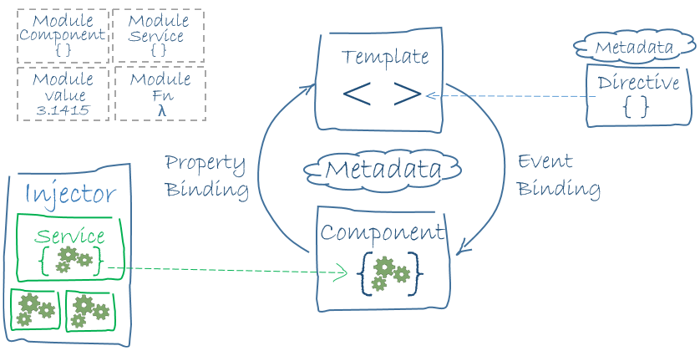
\includegraphics[width=1\linewidth]{angular} 
  \caption{Architettura di Angular}
  \label{fig:angular}
\end{figure}

\subsubsection{Geolocalizzazione}
Come definito nel requisito RF11O l'applicazione deve occuparsi di registrare la posizione dello smartphone. In Ionic, questo è possibile
attraverso l'uso dei plugin. Essendo infatti coinvolta una risorsa hardware dello smartphone, non può essere gestita da Angular. Ho dovuto
ricercare all'interno della documentazione di Ionic e di Capacitor un plugin adatto al nostro scopo. La ricerca non è stata difficile, Ionic
infatti possiede nella sua documentazione una lista di plugin nativi, cioè plugin testati sul framework e compatibili con Capacitor, che
derivano o non sono altro che plugin della community sviluppati per Cordova adattati. \\
\noindent All'interno della documentazione si trovano due plugin che si occupano della localizzazione, Geolocation e Background Geolocation.
Per decidere io e il mio tutor abbiamo constatato che secondo i requisiti dell'applicazione precedente era necessario che l'applicazione
consumasse meno batteria possibile, ma che prendesse continuamente la posizione. Abbiamo quindi optato per Background Geolocation, che
permette di localizzare il telefono anche in modalità background, cioè quando l'applicazione non è aperta nella schermata, o il telefono ha
lo schermo spento. \\
\noindent L'approccio Android per quanto riguarda i processi in background è molto severo. Tutte le applicazioni che avviano processi in
background, infatti, devono avere una notifica che avvisa l'utente che qualcosa sta eseguendo senza che se ne accorgano. Lato sviluppatore
l'applicazione ha bisogno di molti permessi appositi, da inserire in quello che si chiama Manifest, file XML che dichiara tutte le
caratteristiche più importanti dell'applicazione, tra i quali nome e package. \\
Altro rischio rilevato da questo plugin è l'ottimizzazione messa in atto dalle distribuzioni dei vari brand di Android stesso. Sul mio
attuale smartphone, ad esempio, è installato una versione del sistema operativo che si chiama Oxygen OS, questa di default ottimizza tutte
le applicazioni installate. In questo frangente mi è tornato utile il sito Don't Kill My App, il quale per ogni brand indica quali procedure
seguire per disattivare queste ottimizzazioni lato utente.

\subsubsection{Salvataggio offline}
Le applicazioni mobile utilizzano per l'allocazione dati \textbf{SQLite}, una versione ridotta del noto \acrshort{sql}, per la gestione di
\gls{database} relazionali. SQLite permette la creazione di tabelle, form e report e l'interrogazione di questi, tutto all'interno dello
stesso file. Per piccole basi di dati è molto più performante di SQL server e quindi perfetto per il salvataggio di dati di un sistema
mobile. \\
\noindent Anche per questa funzionalità mi sono dovuto affidare a un plugin nativo di Ionic per la gestione di questi database. Per il
debugging e la visualizzazione di questi database ho utilizzato un estensione di Google Chrome, chiamata Stetho.\\
\noindent Nonostante il difficile accesso al database con questo sistema, si è deciso anche che la maggior parte dei dati sensibili, quindi
informazioni personali e chiavi per l'accesso non dovevano essere salvati in locale. 

\subsubsection{Comunicazione con le API}
Come specificato dal requisito RF12O i dati raccolti dall'applicazione dovranno essere inviati al gestionale attraverso le sue \gls{api}.
Angular offre alcune delle sue librerie per comunicare con il server, ma si è preferito utilizzare axios, perché già conosciuto e di facile
utilizzo. Axios è una libreria di Javascript/Typescript che permette di eseguire chiamate \gls{http} di tipo POST/GET/PUT. Supporta il sistema di
Promise di Javascript, quindi la possibilità di fare chiamate asincrone e trasforma tutte le risposte in oggetti JSON, facilmente leggibili
anche non conoscendo la struttura del server. Permette inoltre di impostare un berear token, cioè l'istanza di axios che possiede
l'applicazione deve autenticarsi al server una singola volta, alle chiamate successive non sarà necessario l'invio dei codici per il login
utente.

\section{Progettazione}
\subsection{Login}

\begin{wrapfigure}{l}{0.45\textwidth}
  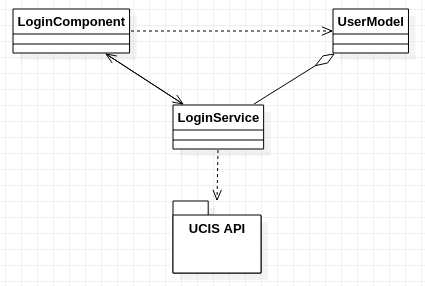
\includegraphics[width=0.9\linewidth]{login} 
  \caption{Semplice diagramma del login}
  \label{fig:login}
\end{wrapfigure}

La prima parte dell'applicazione della quale ci siamo occupati è quella di login. Per fare questo abbiamo optato per una semplice \acrlong{mvc}, con
una classe \textit{User} come modello, che rappresenta le informazioni di un utente, una \textit{View} composta da un semplice form con un
template Angular e un \textit{controller} che si occupa di contattare il server e mantenere l'utente autenticato gestito da un
\textit{service}. \\ \\

\subsection{Creazione e visualizzazione delle attività}
Secondo il requisito RF8O l'applicazione deve permettere all'utente la creazione di un'attività. Il concetto da attività è stato ripreso da
quello già esistente nelle API. Ognuna di esse è formata da:
\begin{itemize}
  \item una categoria individuata da: 
  \begin{itemize}
    \item una \textit{macrocategoria} (es. esercitazioni, addestramento) individuata da un id;
    \item una \textit{sottocategoria} (es. addestramento macerie, ricerca su superficie) individuata da un proprio id e da quello della macrocategoria.
  \end{itemize}
  \item un nome scelto dall'utente;
  \item il cane con cui si svolge l'attività.
\end{itemize}
Inoltre l'applicazione tiene traccia dei seguenti dati:
\begin{itemize}
  \item data di creazione;
  \item data di inizio;
  \item data di fine (se ancora in corso impostata a valore di default);
  \item i nomi delle categorie assiociati agli id;
  \item colore associato alla macrocategoria.
\end{itemize}

Anche in questo caso si è seguito il modello di Angular, molto simile al \acrlong{mvc}. Il \textit{modello} è rappresentato da
una classe attività che possiede come attributi tutte le caratterisitiche precedenti. La \textit{vista} è un \textit{components} Angular compreso di un form e
il \textit{controller} da un servizio chiamato \textit{ActivityService}. Quest'ultimo non gestisce solo la creazione di nuove attività, ma è
un \gls{facade} per tutti components che gestiscono le attività. \\
Un'altra vista importante è quella che permette la visualizzazione della lista delle attività. Qui l'architettura è più complicata e
necessità la spiegazione di cosa sta dietro al \gls{facade}. Infatti secondo il requisito RQ3O l'applicazione deve funzionare anche se
offline, è per questo che la lista delle attività deve essere disponibile anche in assenza di connessione al server del gestionale.
All'apertura dell'applicazione \textit{ActivityService} inizializza un altro servizio con un comportamento simile al \gls{proxy},
\textit{ActivityStore}, che si occupa di leggere nella tabella del database SQLite se sono salvate delle attività e caricarle nei dati
dell'applicazione. Nel frattempo \textit{ActivityStore} inizializza \textit{ActivityFetcher} il quale si occupa invece dell'interrogazione
dell'API, che restituirà una lista di attività se la connessione va a buon fine, oppure un errore.  Nel caso ci sia risposta
\textit{ActivityStore} confronta il risultato con ciò che ha letto dal database e sistema le differenze. Nel caso contrario
\textit{ActivityFetcher} rimane in ascolto della rete dello smartphone (tramite plugin di Ionic) e una volta trovata, rilancia
l'interrogazione al server. 

\subsection{Registrazione Attività}
La parte di registrazione delle attività risulta essere molto più complicata per alcuni motivi:
\begin{itemize}
  \item continuo invio di dati al gestionale per requisito RF11O;
  \item registrazione anche se l'app è in background;
  \item registrazione anche se lo smartphone è offline.
\end{itemize}
Questi punti hanno richiesto molto per essere modellati e più volte l'architettura di questa componente è stata modificata. \\
\noindent Ad alto livello quello che si tenta di fare è mettere in comunicazione il plugin di Ionic che riceve i dati sulla posizione e inviarli al
gestionale. Qui entrano in gioco due servizi di Angular: uno si occupa di ricevere, registrare e salvare i log nel database locale
dell'applicazione; un altro che si occuperà di verificare la rete periodicamente, e, nel caso fosse presente, procederà a caricare i log che
trova all'interno della memoria. La caratteristica che devono avere i due servizi, che chiameremo \textit{ActivityRecorder} e \textit{uploader}, è di dover
essere eseguibili anche in background. Inoltre l'uploader dovrà occuparsi di sincronizzare i propri processi, dato che potrà inviare una
sola richiesta alla volta. 

\section{Verifica}
Il processo di verifica e validazione è stato avviato dopo la codifica di una \gls{Product Baseline} funzionante. 
\subsection{Analisi statica}
Dato che la maggior parte dell'applicazione è stata codificata in Typescript gli strumenti utilizzati per la verifica sono quelli standard
del linguaggio, integrati anche nell'\gls{ide}. Per l'analisi statica si è utilizzato TSLint, reperibile al link: \\
\begin{center}
  \url{https://palantir.github.io/tslint/}.
\end{center}
\subsection{Analisi Dinamica}
Per i test dinamici sull'interfaccia si è usato un framework apposito di Angular, Protractor anch'esso reperibile al link: \\
\begin{center}
  \url{https://www.protractortest.org/#/}.
\end{center}
I test sono definiti come \textit{behaviour driven}, vengono definiti degli input sull'interfaccia e dei comportamenti aspettati.
L'applicazione viene poi lanciata sul browser per verificare che l'output dell'applicazione sia corretto.

\subsection{Analisi umana}
Alcune delle componenti dell'applicazione, purtroppo, non sono stati testati in modo automatico, perchè non esistente alcuno strumento per
farlo. È il caso del test per il plugin di geolocalizzazione, non era possibile testarlo con nessun tool e questo si è tradotto in prove
empiriche sul campo, durante gli spostamenti per andare in ufficio, ad esempio.